\chapter{Desenvolvimento}
\label{c.desenvolvimento}

\section{Base de dados}

Para este trabalho foi utilizada uma base de dados fornecida pela \textit{University of New Brunswick} \cite{unbdataset}. Esta base vem sendo utilizada em vários estudos recentes da área, como \cite{iscx1} e \cite{rna1}, e portanto sua utilização é de extrema relevância. Foram fornecidos três arquivos no formato PCAP, sendo um voltado para a fase de treinamento e dois para testes. No entanto, os arquivos de teste apresentaram problemas, com ambos não podendo ser processados pelo programa.

Um deles apresentava problemas de desordenamento dos pacotes, que ao tentar ser resolvido levou a uma descaracterização dos dados, como por exemplo valores de duração negativos, algo que não é possível por se tratar de uma medida de tempo. Já o segundo apresentou problemas de corrompimento, que também impediram seu processamento.

Sendo assim, todo o desenvolvimento deste trabalho, assim como seus resultados, serão baseados somente no conjunto de treino fornecido, utilizando a técnica de \textit{Hold-out} explicada anteriormente.

\section{Geração de fluxos de rede}
\label{d.fluxo}

Para que os estimadores pudessem trabalhar no conjunto de dados, foi preciso primeiro passar os arquivos de pacotes por um gerador de fluxos bidirecionais, um programa capaz de analisar todos os pacotes e extrair características dos fluxos de rede presentes nele.

Para este fim, foi utilizado o programa \textit{flowtbag}, uma ferramenta \textit{open-source} desenvolvida na linguagem \textit{Go}, disponível no \textit{GitHub} \cite{flowtbag}. A interface de utilização do programa se dá através da linha de comando, onde são passados o caminho para o arquivo de pacotes a ser analisado, e o caminho para onde o arquivo final, no formato CSV, deve ser salvo.

\begin{figure}[h]
\caption{\small Gerando arquivo de fluxos bidirecionais com a biblioteca \textit{flowtbag}.}
\centering
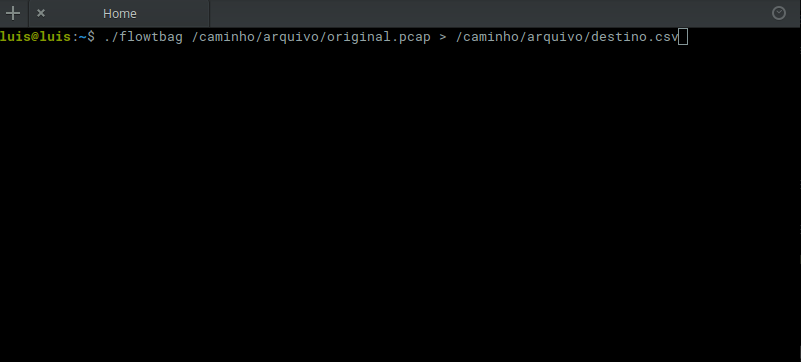
\includegraphics[scale=0.50]{figs/exemplo-flowtbag.png}
\label{f.exemplo-flowtbag}
\legend{\small Fonte: Elaborada pelo autor.}
\end{figure}

O arquivo CSV que o programa cria contém uma tabela onde as linhas representam cada fluxo de rede, e as colunas representam as características extraídas. Ao todo são 44 características,sendo que as cinco primeiras são as que definem um fluxo: IP de origem, IP de destino, Porta de origem, Porta de destino, e Protocolo.

Além das acima citadas, se fazem presentes no conjunto:

\begin{itemize}
    \item Total de Bytes;
    \item Total de Pacotes;
    \item Total de bytes alocados para cabeçalhos de pacote;
    \item Mínimo/Máximo/Média/Desvio Padrão da média de: menor pacote enviado, IAT, tempo ativo, tempo ocioso, ocorrências da flag \textit{Push}, ocorrências da flag \textit{Urgent};
\end{itemize}

As características de fluxo acima, com exceção de tempo ativo e tempo ocioso, são dividas em dois tipos: \textit{forward}, indica os valores correspondentes ao que foi enviado do IP de origem ao IP de destino, e \textit{backwards} indica o contrário, ou seja, o que o destinatário enviou a quem iniciou a conexão. Por exemplo, o número de pacotes trocados durante o fluxo é representado por dois valores, \textit{totalfpackets} e \textit{totalbpackets}, onde o primeiro indica quantos pacotes foram transmitido na direção \textit{forward} e o segundo na direção \textit{backward}. 

\section{Processamento de dados}

Depois de gerados o arquivo CSV, foi preciso fazer uma análise e processamento dos dados de forma que eles fossem usados pelos estimador. Para isto, foram utilizadas varias funcionalidades da biblioteca Pandas.

O programa gerador utilizado faz o processamento de conexões que utilizam o protocolo TCP e UDP, porém como o foco do projeto é analisar o fluxo de botnets do protocolo IRC, que por sua vez utilizam o protocolo TCP para transporte \cite{livadas2006usilng}, como explicado anteriormente, foi feita uma filtragem para que somente os protocolos desse tipo fossem mantidos na base de dados. 

Os fluxos de protocolo TCP eram representados pelo número 6, enquanto o número 17 representava os fluxos UDP. Dessa maneira, foi necessário somente filtar os fluxos com número de protocolo igual a 6.

Depois de eliminado os fluxos que não iriam ser utilizados, foi feita a rotulação dos dados, que consiste em atribuir para cada uma das linhas da tabela um valor que indica se aquele fluxo é de botnet ou não. Para essa tarefa, foram utilizados dois recursos: uma lista de IP's fornecida juntamente com a base de dados que informa o IP usado pelas botnets, e uma tabela pertencente ao estudo desenvolvido em conjunto com a base, que informa quais são as botnets presentes em cada conjunto.

Com essas informações, foi possível então desenvolver um método que iterasse por toda a tabela verificando se os IPs dos fluxos correspondiam aqueles dos ataques. Em caso positivo, era atribuído o valor 1, e 0 caso contrário.

\begin{figure}[h]
\caption{\small Rotulação dos fluxos.}
\centering
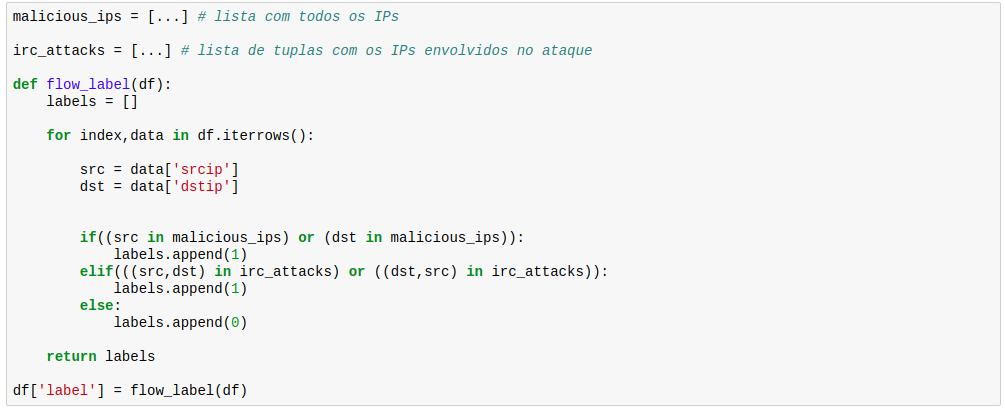
\includegraphics[scale=0.40]{figs/rotulacao-dados.png}
\label{f.rotulacao-dados}
\legend{\small Fonte: Elaborada pelo autor.}
\end{figure}

Além disso, foram também eliminados todos os fluxos de Botnets que não fossem do protocolo IRC, evitando assim com que houvesse interferência dessas informações nos resultados, tendo em vista que apesar de utilizarem protocolos diferentes, as redes ainda podem compartilhar certos tipos de comportamentos gerais, o que poderia acarretar em predições equivocadas.

Por fim, foi observado que a distribuição de fluxos por classe estava desbalanceada, com 86695 fluxos da classe 0 e somente 6379 da classe 1. Como os classificadores costumar trabalhar melhor com distribuições de dados balanceadas,foi aplicada a técnica do \textit{Undersampling}, diminuindo o número de amostras da classe 0 para o mesmo número de amostras da classe 1.

Foi necessário também criar algumas colunas de dados que não foram geradas automaticamente pelo programa. Como citado na seção anterior, o programa gerador divide as características em dois tipos, \textit{forward} e \textit{backward}, o que permite uma maior flexibilidade ao se trabalhar com os dados, porém exige que alguns cálculos sejam feitos para se gerar certas características mais gerais.

Foi preciso então, criar métodos capazes de trabalhar com os valores presentes para gerar alguns dados que foram utilizados em pesquisas anteriores da área. A tabela 1 mostra quais são essas características e como elas foram calculadas:

\begin{table}[ht]
\centering
\begin{tabular}{|c p{10cm}|l p{10cm}}
\hline
\textbf{\small Característica} & \textbf{\small Fórmula geradora}\\\hline \hline
{\small Total de Bytes} & {\small Soma dos bytes enviados em ambas as direções}\\\hline
{\small Total de pacotes} & {\small Soma dos pacotes enviados em ambas as direções}\\\hline
{\small Total de Bits} & {\small Número total de bytes multiplicado por 8 (1 byte = 8 bits)}\\\hline
{\small Bytes por pacote} & {\small Razão entre o Total de Bytes e Total de pacotes}\\\hline
{\small Bytes por segundo} & {\small Total de bits dividido pela duração do fluxo}\\\hline
{\small Pacotes por segundo} & {\small Total de pacotes dividido pela duração do fluxo}\\\hline
{\small Média de IAT} & {\small Média da soma dos valores IAT médios}\\\hline
{\small Bytes por segundo} & {\small Total de bits dividido pela duração do fluxo}\\\hline
{\small Média de variância de IAT} & {\small Média dos desvio padrão de IAT ao quadrado}\\\hline
{\small Porcentagem de pacotes enviados} & {\small Razão entre o número de pacotes enviado na direção \textit{forward} e o número total de pacotes do fluxo}\\\hline
{\small IOPR} & {\small Razão entre a quantidade de pacotes na direção \textit{backward} sobre a quantidade da direção \textit{forward}}\\\hline
{\small Média de tamanho de payload} & {\small Número de bytes total do fluxo menos a soma de bytes dos headers em ambas as direções, depois dividido pelo número de pacotes}\\\hline
\end{tabular}
\caption{Fórmulas utilizadas para geração de características.}
\label{t.caracteristicas-geradas}
\end{table}

\begin{figure}[h]
\caption{\small Exemplo de geração de colunas.}
\centering
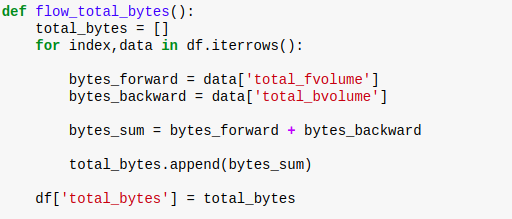
\includegraphics[scale=0.40]{figs/exemplo-geracao-coluna.png}
\label{f.exemplo-colunas}
\legend{\small Fonte: Elaborada pelo autor.}
\end{figure}

A figura \ref{f.exemplo-colunas} mostra o processo básico para a geração dessas colunas, utilizando como exemplo a coluna "Total de bytes". As linhas da tabela inteira são percorridas, as características necessárias para a geração são obtidas, as operações efetuadas e o resultado é adicionado para uma lista. Por fim, essa lista era adicionada no conjunto de dados como uma nova coluna. O processo é o mesmo para todas as outras características, alterando-se somente os cálculos e valores utilizados.

Por fim, foram removidas algumas colunas em que todos os valores eram 0, ou seja, dados que o gerador não foi capaz de obter nenhuma informação no conjunto de dados. Estas colunas foram as seguintes: Desvio padrão de tempo ativo de conexão, tempo mínimo de ociosidade na conexão,média de tempo de ociosidade na conexão, tempo máximo de ociosidade na conexão, desvio padrão do tempo de ociosidade na conexão, número de vezes em que a \textit{flag Urgent} foi enviada da origem para o destino, e número de vezes em que a \textit{flag Urgent}  foi enviada do destino para a origem.

Junto com estas, também foram removidas colunas que não são relevantes para os algoritmos, IP/Porta de origem e de destino e protocolo, que apesar de terem sido muito úteis para a rotulação e filtragem, não serão utilizados para a tarefa de classificação, entre outras.

\begin{figure}[h]
\caption{\small Removendo colunas nulas e desnecessárias para a classificação do conjunto.}
\centering
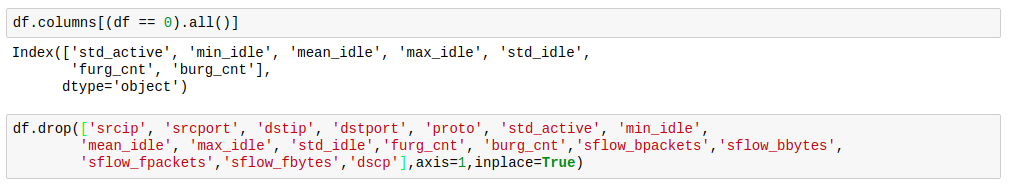
\includegraphics[scale=0.40]{figs/drop-colunas.png}
\label{f.drop-colunas}
\legend{\small Fonte: Elaborada pelo autor.}
\end{figure}

\section{Execução dos algoritmos}

Com os dados preparados, é possível então usá-los para treinar os algoritmos. Contando todas as colunas válidas do gerador e as características geradas manualmente e desconsiderando a coluna de rótulos, têm-se 39 colunas de características.

No entanto, não é viável executar os estimadores com todas, mas sim tentar encontrar um subconjunto destas que melhor caracterize o problema. Para este fim, foram aplicadas duas abordagens:

\begin{itemize}
    \item Busca de força bruta com base em dados de pesquisas anteriores: foram utilizadas somente as características presentes em trabalhos da área, e através de uma pesquisa de força bruta rodar todas as combinações delas com todos os algoritmos e assim desta maneira encontrar o melhor conjunto de características para cada classificador;

    \item Busca utilizando um algoritmo específico de seleção de características: o Scikit possui vários algoritmos para seleção de características, que buscam encontrar dado um conjunto a melhor combinação. Para este trabalho, será utilizado o RFE no conjunto inteiro de dados, tanto os do gerador de fluxo quanto os criados com base em estudos anteriores. 
\end{itemize}

\subsection{Busca de força bruta com base em dados de pesquisas anteriores}
\label{ss.dados-hist}

Para essa primeira abordagem, a ideia era testar todas os subconjuntos possíveis de características com todos os estimadores, e verificar qual combinação de características seria melhor com cada um deles.

Para obter as combinações de características do conjunto, foi utilizada a biblioteca \textit{itertools} do Python. A figura x mostra o processo de geração dos subconjuntos, aonde foi definido um numero mínimo de características por conjunto de 4. O resultado gerado é uma lista contendo todas as combinações. Ao fim do processo, foram geradas 1816 possibilidades.

\begin{figure}[h]
\caption{\small Gerando combinações com a biblioteca \textit{itertools}.}
\centering
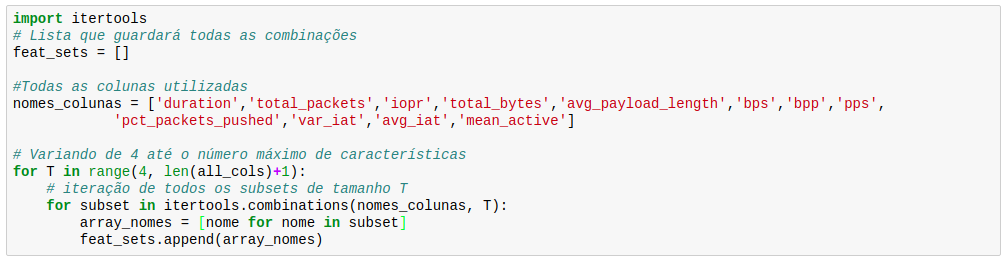
\includegraphics[scale=0.40]{figs/exemplo-itertools.png}
\label{f.exemplo-itertools}
\legend{\small Fonte: Elaborada pelo autor.}
\end{figure}

Depois, todas as combinações foram processadas por todos os estimadores, e as acurácias dos modelos obtidas. Foram criados vetores contendo instâncias de todos os estimadores a serem utilizados no trabalho, e depois este era percorrido, de maneira que a cada iteração o modelo fosse treinado e uma predição fosse obtida, salvando em uma tabela a acurácia e qual conjunto de dados foi usado. A figura x mostra o método utilizado para este processo. 

Ao fim deste processo, foi possível filtrar os dados da tabela pelas maiores acurácias de cada estimador, e assim encontrar o subconjunto ótimo para este, assim como a acurácia obtida.

\subsection{Utilizando o algoritmo Recursive Feature Elimination}
\label{ss.dados-rfe}

A ideia desta abordagem é utilizar o algoritmo RFE em todos o conjunto de dados, e dessa maneira observar quão eficaz são os dados utilizadas historicamente na área na tarefa de classificação, e também identificar se algumas das fornecidas pelo gerador são eficazes nesse processo, através do processo de observação das características escolhidas pelo algoritmo. 

Além disso, outro ponto dessa abordagem é verificar se as características utilizadas nos estudos anteriores possuem grande representatividade dado todo o conjunto de características, ou seja, se elas serão escolhidas pelo algoritmo.

O Scikit implementa o RFE em conjunto com a técnica de CV, para todos os números possíveis de parâmetros. Dessa maneira, é possível identificar não só um número fixo de características mas também encontrar qual o número ideal. Para utilizá-lo, passa-se como argumento uma instância do classificador desejado, e depois aplica-se a função \textit{fit} com um conjunto de treino, para que ele encontre o subconjunto ótimo.

Depois de encontrado, é possível acessar tanto o estimador quanto as características do conjunto de maneira ranqueada. Todas as características escolhidas são atribuídas o valor 1, e dessa maneira é possível tanto definir quais as características ótimas quanto já executar predições com o estimador que a estrutura fornece.  

\subsection{Otimização de Hiper-parâmetros}

Obtidos os melhores conjuntos de características para todos os estimadores utilizando as duas abordagens, o último passo a ser feito nesta etapa é aplicar a técnica de \textit{Grid Search} para otimizar hiper-parâmetros no algoritmo de SVM, que como explicado anteriormente na seção \ref{c.fundamentacao} é muito depende da otimização de seus hiper-parâmetros para obter melhores resultados.

O Scikit implementa a tecnica de \textit{Grid Search} em conjunto com o CV. A interface de utilização é muito parecida com a de um estimador normal, com a diferença de que deve ser passado também um dicionário com os parâmetros que serão testados e seus respectivos valores.

\begin{figure}[h]
\caption{\small Utilização do \textit{Grid Search} no Scikit.}
\centering
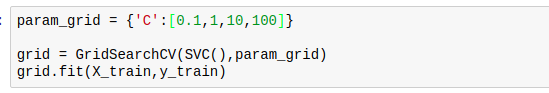
\includegraphics[scale=0.80]{figs/gridsearch.png}
\label{f.exemplo-gridsearch}
\legend{\small Fonte: Elaborada pelo autor.}
\end{figure}

Foram testados os Kernels Linear, RBF e Sigmoidal. Foram feitas tentativas de cálculo com o Kernel Polinomial, no entanto foram apresentados problemas de execução específicos que impediram a obtenção de resultados.

Foram testados os seguintes valores:

\begin{itemize}
    \item C: {0.1,1,10,100};
    \item $\gamma$: {0.0001,0.001,0.01,0.1,1};
    \item Coeficiente $r$, específico do Kernel Sigmoidal: {-1,0,1}.
\end{itemize}

